% Chap 1. Introduction
\chapter{緒論}
\label{c:intro}
\section{研究動機與目的}
美國國防部高等研究計劃署(Defense Advanced Research Projects Agency,DARPA)
分別於2004、2005與2007年舉辨了無人車輛競速大賽,各參賽隊伍運用各種感測器儀器,
定位導航技術及影像處理技術等挑戰橫越沙漠和穿越城市。
而Google公司也在2011年時也發表了自行研發的無人自走車,
可見現今人工智慧的發展讓自主式無人載具成為目前廣為研究的課題,
而基於這些影響,本實驗室也開始投入研究無人自走車的領域。

本實驗室目前已擁有一輛使用四驅越野搖控車作為底盤架構的Yun-Trooper實驗平台,
先前也使用此平台完成了許多研究:
陳維懋~\cite{Chen:2011:Thesis}使用電腦視覺的方式來完成自動巡航,
但由於電腦視覺容易受到環境干擾,
呂明修~\cite{Liu:2012:Thesis}使用全球衛星定位系統(GPS)
及慣性量測單元(IMU)取代電腦視覺系統來完成自動巡航。

第一代Yun-Trooper,如圖~\ref{f:YunTrooperI}~所示,
使用工業用電腦主機板搭配Windows XP作業系統作為決策中心,
加上電腦視覺所需要的攝影機與影像擷取卡,
其體積龐大且重量較重,造成巡航速度降低與耗電量增加。
而本論文使用原先的底盤開發了第二代實驗平台Yun-Trooper II,
如圖~\ref{f:YunTrooperII}~所示,其使用嵌入式單板電腦搭配Linux作業系統,
並且簡化了所需要的週邊配備,使得體積與重量大幅降低,開發成本也大幅下降。
\begin{figure}[h!]
	\centering
	\begin{subfigure}[b]{0.45\textwidth}
		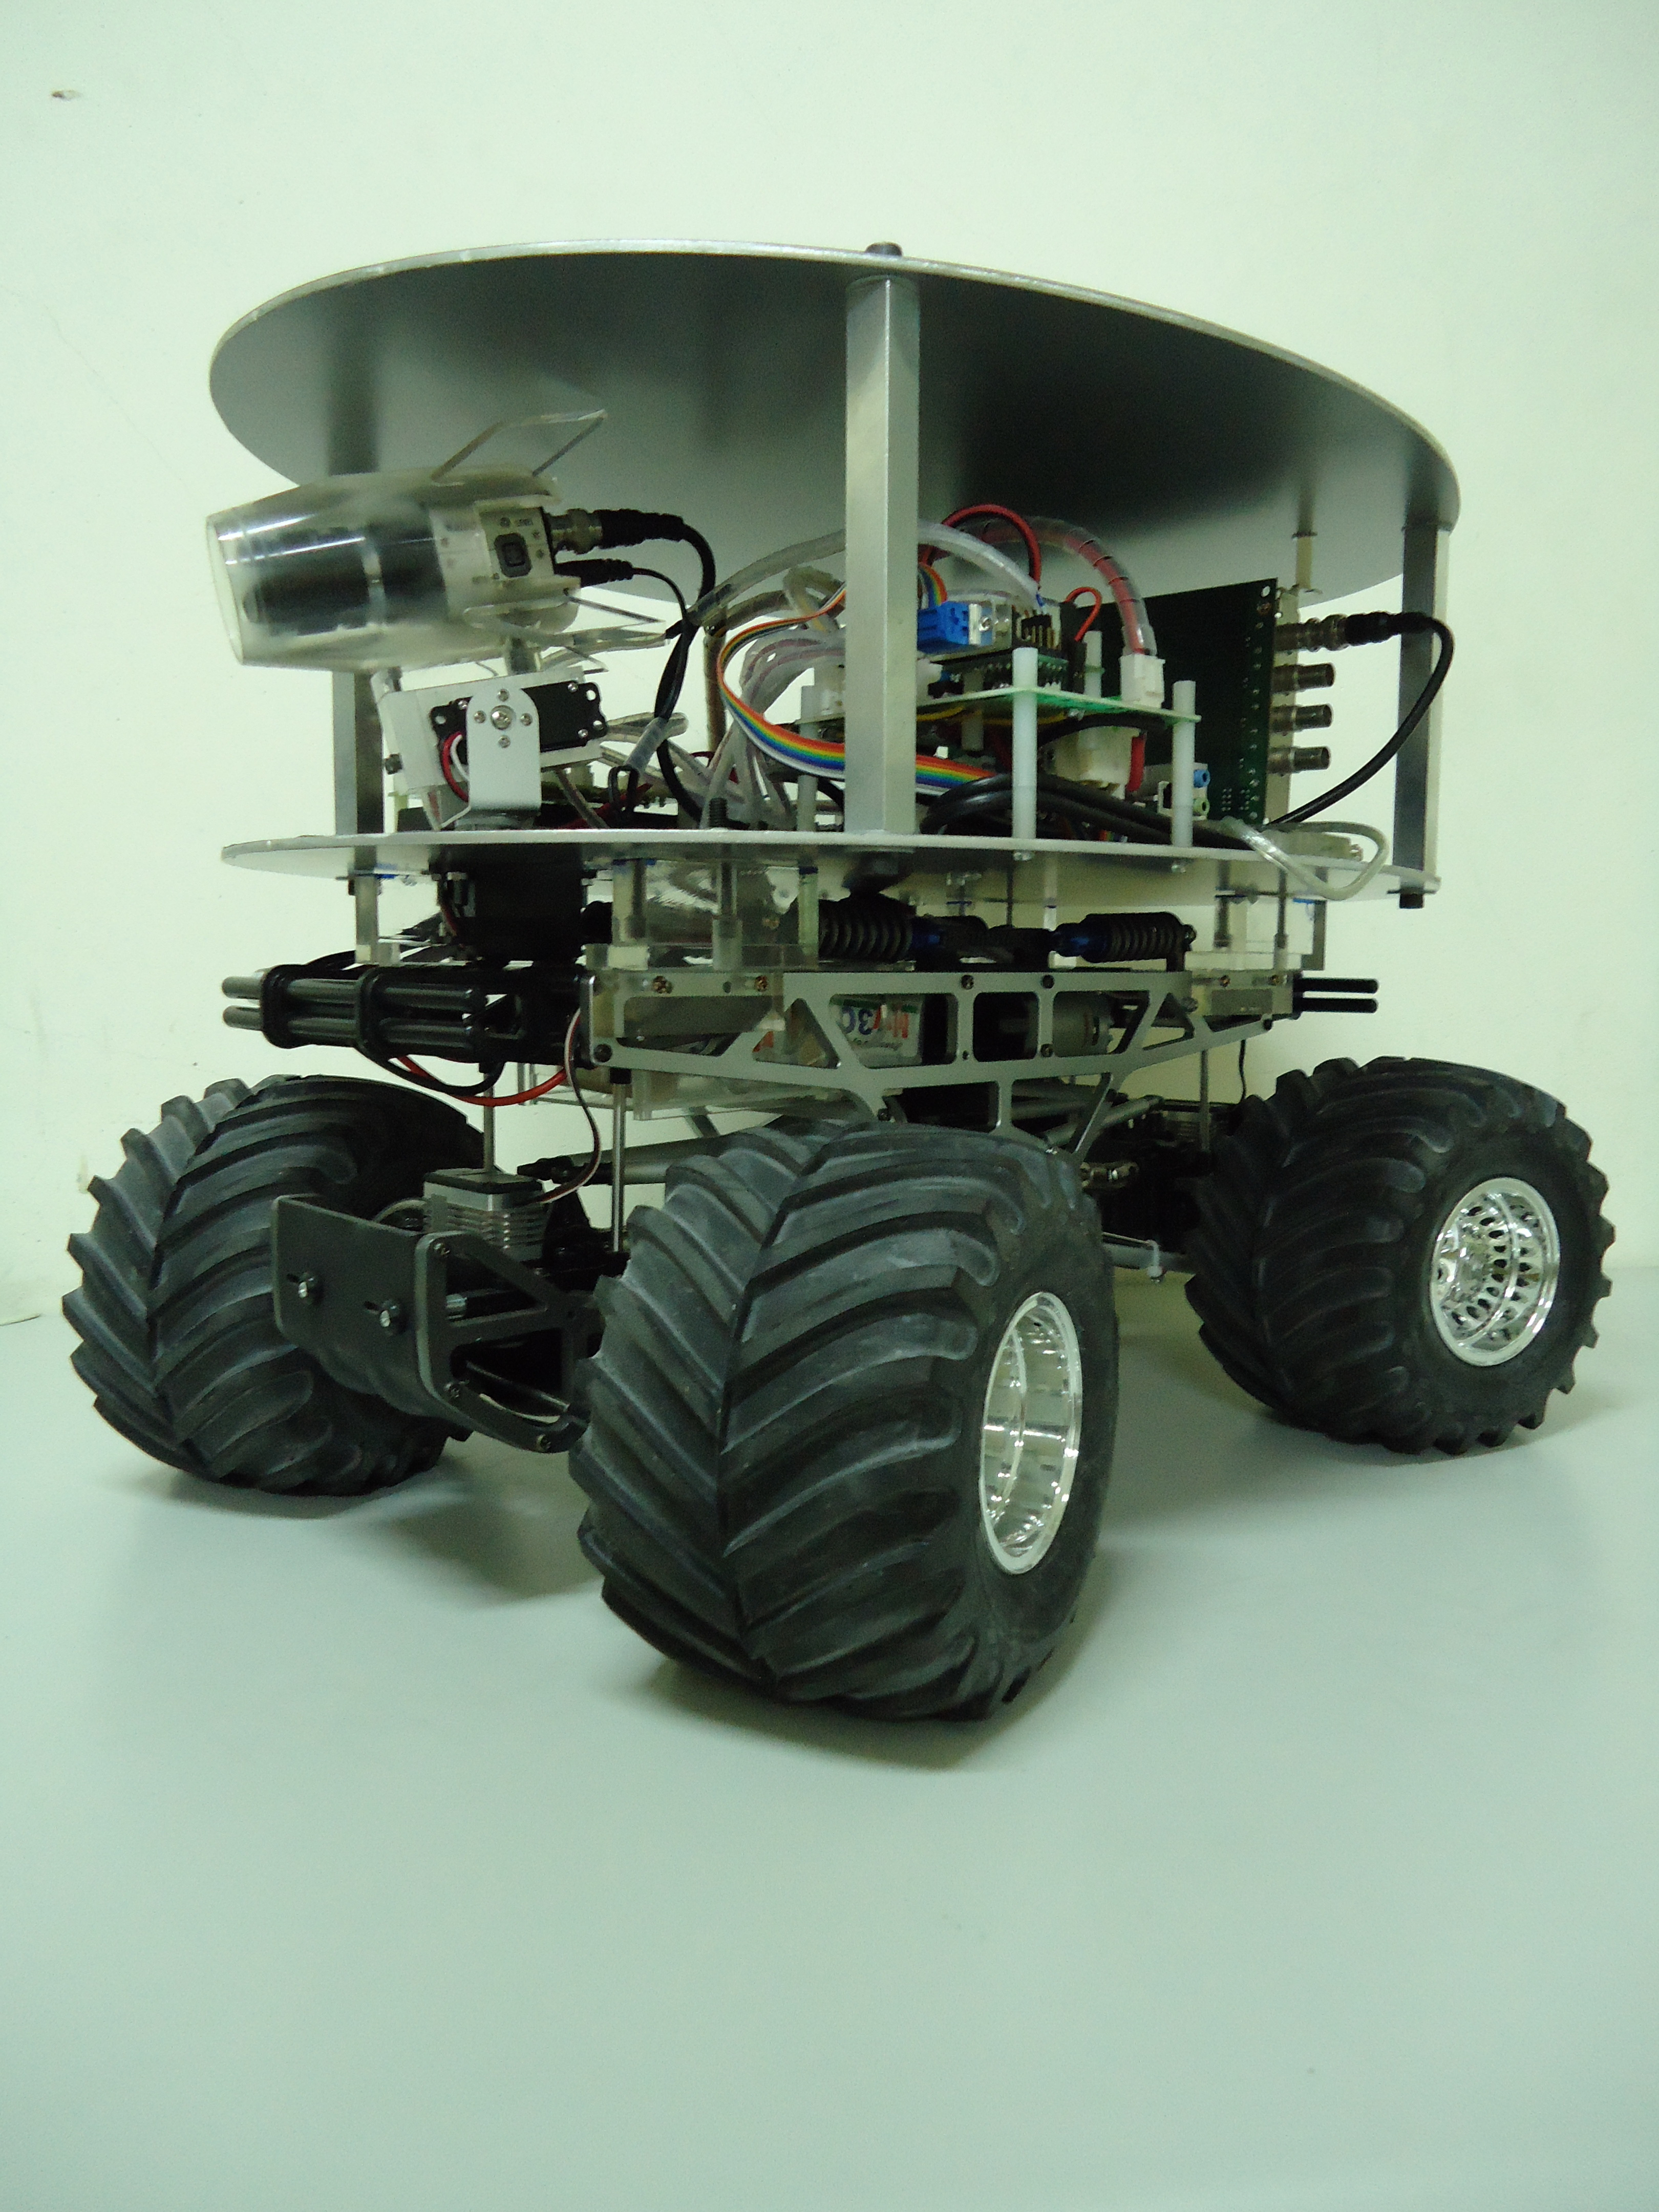
\includegraphics[width=\textwidth]{figures/YunTrooper}
		\caption{Yun Trooper}
		\label{f:YunTrooperI}
	\end{subfigure}
	\begin{subfigure}[b]{0.45\textwidth}
		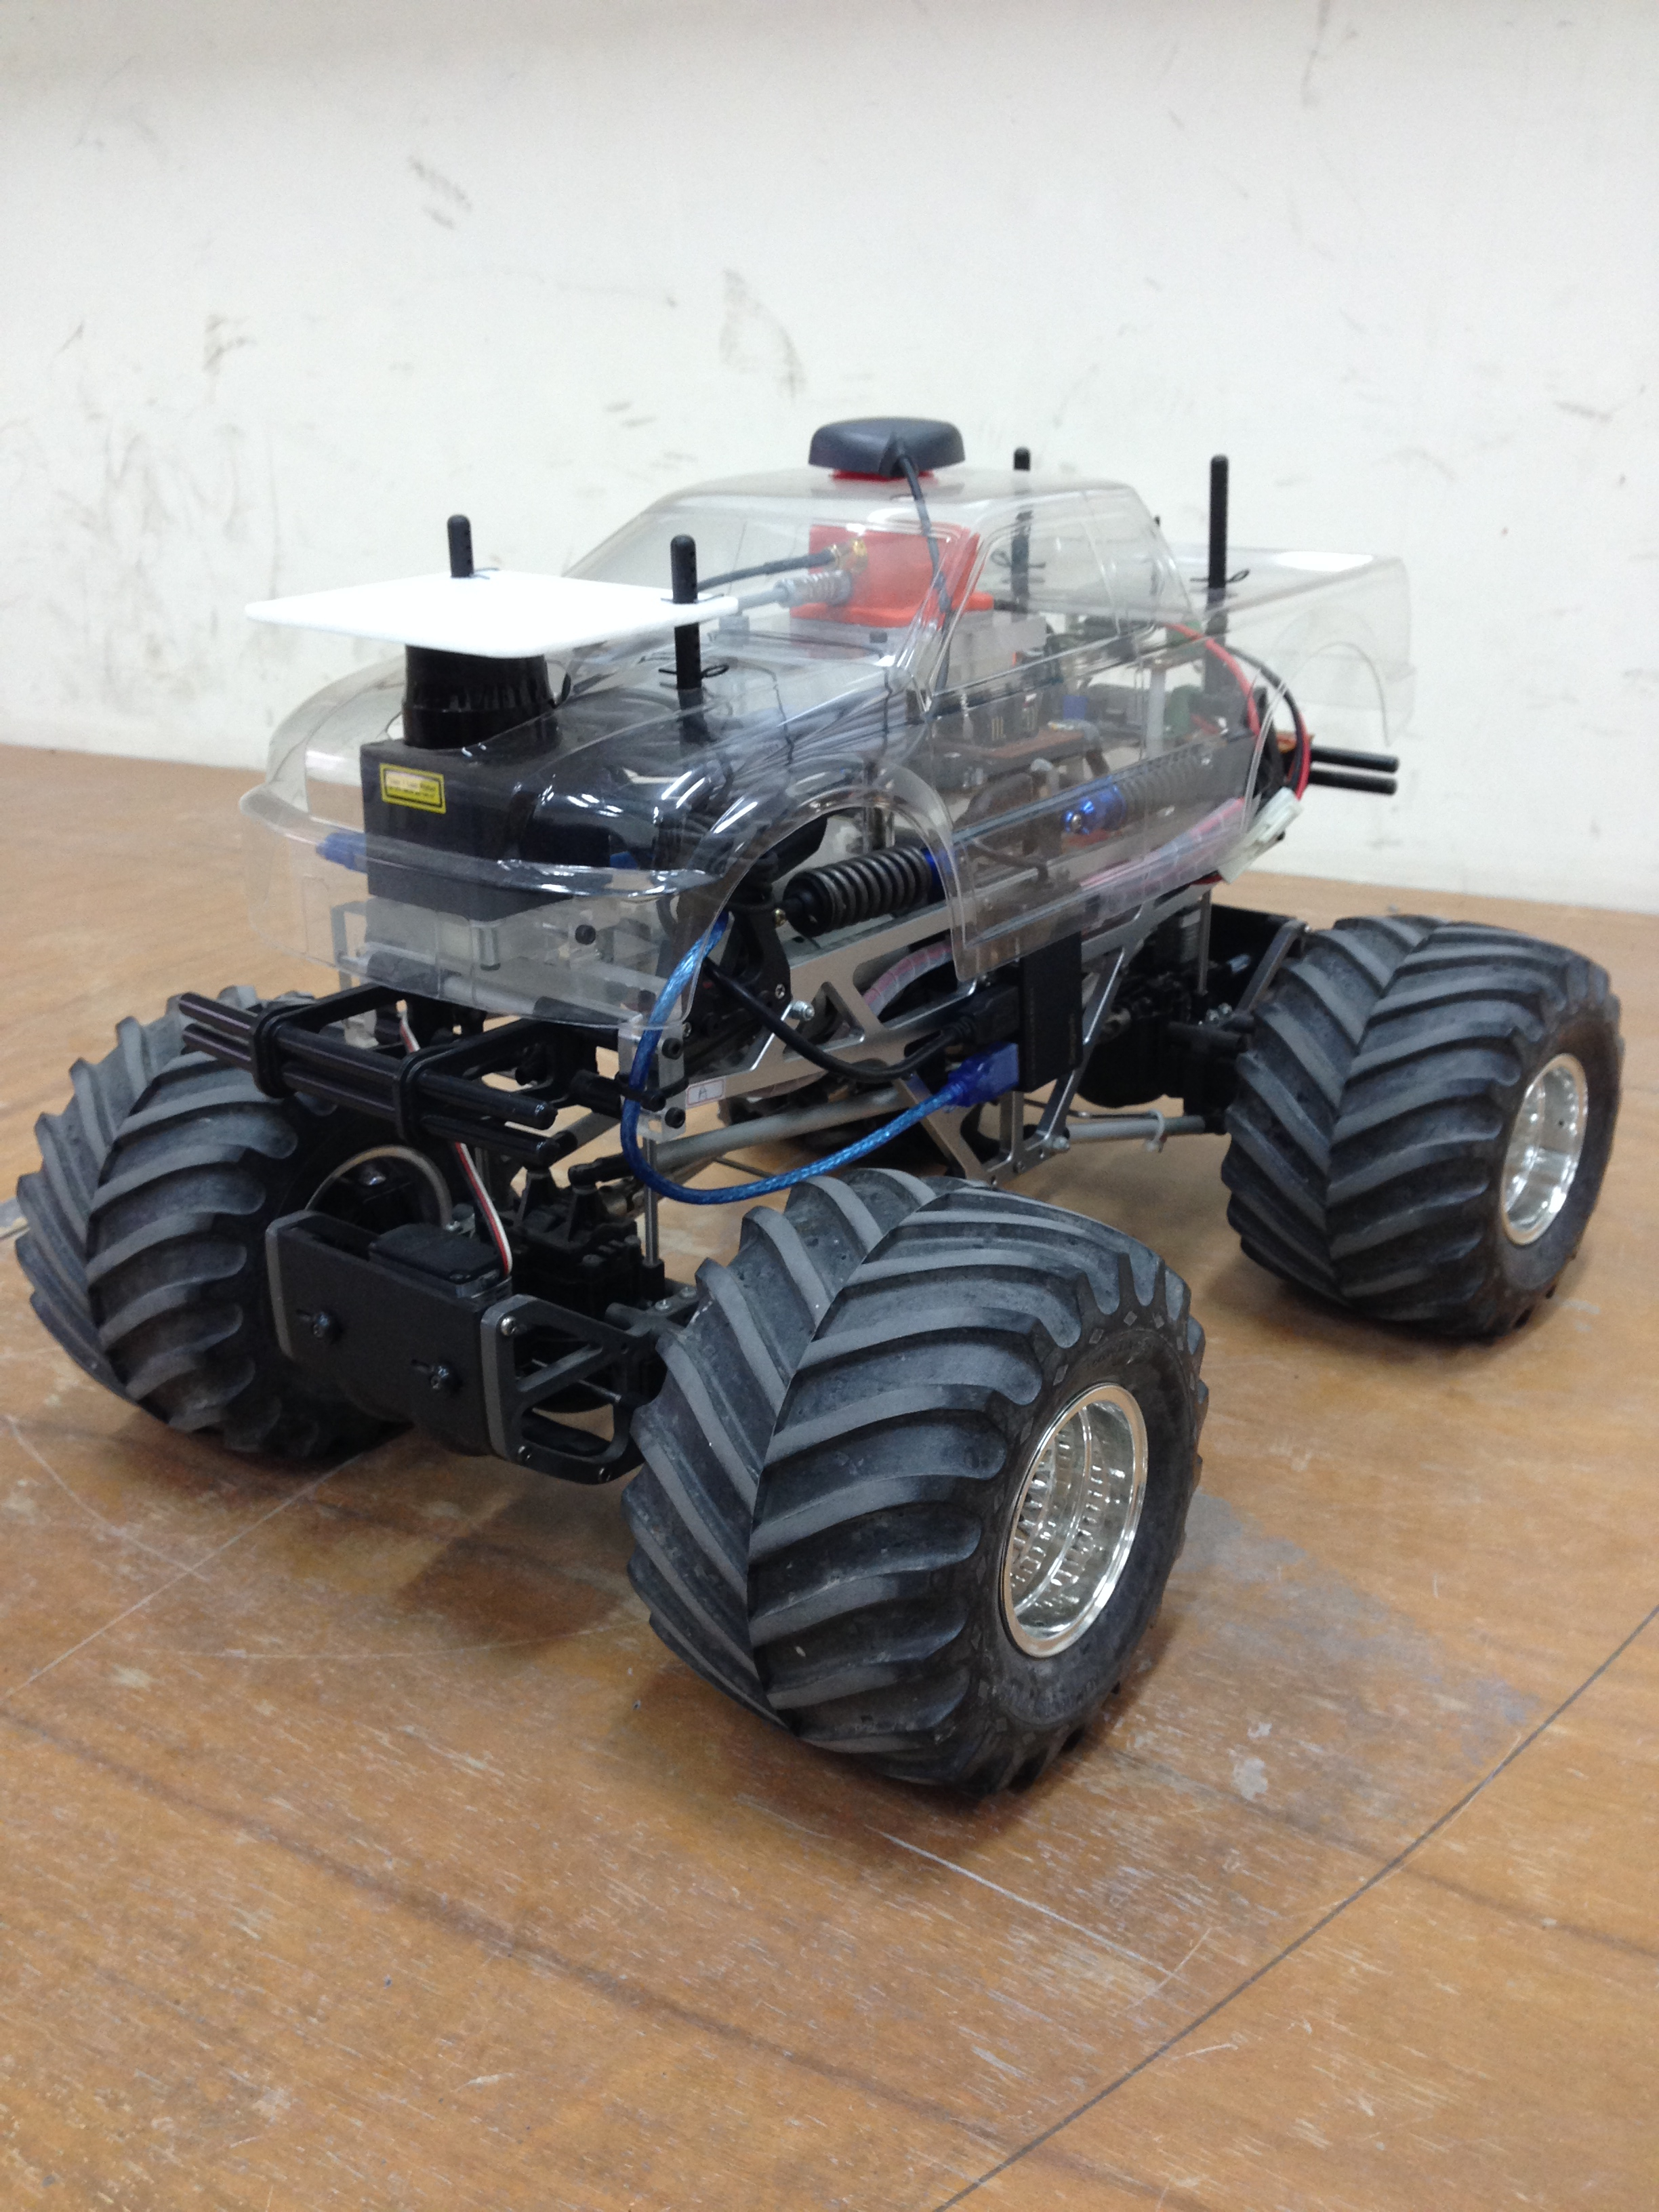
\includegraphics[width=\textwidth]{figures/YunTrooperII}
		\caption{Yun Trooper II}
		\label{f:YunTrooperII}
	\end{subfigure}
	\caption{Yun Trooper比較}
\end{figure}

本論文所開發的Yun-Trooper II裝置有無線通訊模組,
因此使用者可在遠端以個人電腦或其它工具控制Yun-Trooper II的一切功能。
使用者可以將導航目標點以經緯度的方式,直接手動輸入至電腦並傳送給Yun-Trooper II;
或是以搖控的方式將Yun-Trooper II事先移動至導航目標點,並使用車輛裝置的GPS記錄該點之經緯度,
之後便可依導航目標點的傳送或記錄順序,利用姿態量測系統(AHRS)計算導航方向,依序導航至各個目標點。
而導航過程中將使用光學雷達(LiDAR)量測環境的變化,同時規劃出安全的路徑以避開障礙物,避免碰撞。

\section{研究方法與文獻回顧}
本章將依Yun-Trooper II的研究方法及過程做出相關的文獻回顧。

\subsection{導航方向計算}
本論文提出的方法利用車輛本身位置與目標位置之間的相對關係,以及車輛的方位角,
計算出相對距離及角度差,並做為車輛控制法則的參數。
而GPS所量測到的經緯度是以WGS84大地基準(World Geodetic System 1984 Datum)
為參考座標系所得到的座標位置~\cite{Xsens:2012:MTiG_Manual}。
WGS84為一橢球面(Ellipsoid),量測到的每一個經緯度都代表此橢球面上的一點
~\cite{El-Rabbany:2006:IntroGPS},
因此若要計算兩組經緯度之間的最短距離與方向,就必須考慮橢球面與圓球面之間的差異,
才能得到正確的數值。這個最短距離就稱為測地線(Geodesic)\cite{Karney:2013:Algorithms_for_Geodesics}。

自19世紀以來便有許多著名的數學家著手解決這個問題,例如勒讓得(Legendre, A. M.)、
貝索(Bessel, F. W.)及高斯(Gauss, C. F.)等。而由於現代電腦運算速度的提昇和數值方法的演進,
Karney~\cite{Karney:2013:Algorithms_for_Geodesics}提出了適用於現代電腦的相關演算法。
本論文使用這位作者所開發的GeographicLib函式庫~\cite{website:GeographicLib}來做此方面的運算,
增加運算效能以及縮短開發的時間。

\begin{comment}
由於本身的自轉與重力的不均勻分布,地球是一個相當不平整的曲面,
因此要精確計算地球上兩點之間的距離相當困難。
為了解決此類問題,大地測量學家(Geodesist)透過數學建立一標準曲面(例:球面),
做為地球的參考基準面,用以估測地球的不規則形狀。對GPS這樣高精度的測量儀器來說,
雙軸橢球(Biaxial Ellipsoid)相對於球面能夠更加準確的去描述地球基準面,
同時也能保持一定的計算容易度~\cite{El-Rabbany:2006:IntroGPS}。
做為基準面的參考橢球是將一橢圓以其短軸為旋轉軸,旋轉一圈後所得到的曲面。
與橢圓相同,一個橢球可用兩個參數來定義,可以是長軸$a$與短軸$b$,
或是長軸$a$與扁率$f$,其中扁率(Flattening)定義為$f = 1 - (b/a)$~\cite{El-Rabbany:2006:IntroGPS}。

一個明確定義了其原點及旋轉方向的參考橢球稱為大地基準(Datum),
\end{comment}

\subsection{路徑規劃}
依路徑的規劃範圍可分為全域路徑規劃與部份路徑規劃(Global/Local Path Planning),
有時也會以路徑規劃(Path Planning)與避障(Obstacle Avoidance)
的名稱來區別~\cite{Siegwart:2004:IAMR}。
全域路徑規劃是藉由地圖的輔助,根據不同的需求(最短路徑、最少轉向、最容易通過等)
與地圖上已知的障礙物,像是建築物、走廊等,規劃出不同的路徑;
部分路徑規劃則是利用感測器所量測到的環境資訊,對當下的環境變化做出反應,
避開地圖上沒有出現或是隨時間改變的障礙物,例如隨機放置的紙箱、路人等等。
而自走車必須要同時具備兩種路徑規劃演算法,才能夠得到最高的導航效率。

然而Yun-Trooper II並無法預先得知地圖資訊,因此在全域路徑規劃方面,
如上一小節所述,只有計算兩點之間的直線距離與導航方向。
在區域路徑規劃方面,大部分的演算法都是將感測器所得到的資訊,
從實際的二維或三維空間轉換至各種不同的組態空間(Configuration Space)以簡化資訊量,
並且從該空間透過不同的方法計算最佳路徑,以避開障礙物。

Artificial Potential Field~\cite{Khatib:1985:APF}將環境資訊轉換為一虛擬力場,
讓目標對機器人施加吸引力,而障礙物則對其施加排斥力,而合力即為自走車應走的方向。
Vector Field Histogram~\cite{Borenstein:1991:VFH}
使用極座標的方式取得環境資訊並建立直方圖,找出足夠讓機器人通過的空間,並計算其轉向角度。
Curvature Velocity Method~\cite{Simmons:1996:CVM}
假設機器人的運動軌跡為圓弧,並將障礙物簡化為圓形,接著找出能夠讓機器人前進最長距離的一條路徑。
Dynamic Window Approach~\cite{Thrun:1997:DW}
同樣假設機器人的運動軌跡為圓弧,並將環境資訊轉換至速度空間(Velocity Space),
接著考慮動態拘束後找出可行方向,並計算最佳解。

由於Yun-Trooper II不具速度感測器,本論文採用增強後的Vector Field Histogram演算法:
Vector Field Histogram Plus(VFH$^+$)~\cite{Ulrich:1998:VFHPlus}做為基礎,
改進其功能使之能夠利用光學雷達得到的資訊。

\section{論文架構}
本論文共有六章,除本章外,第二章描述Yun-Trooper II所使用的硬體架構;
第三章介紹導航所使用的演算法;
第四章介紹Yun-Trooper II的程式架構及控制法則;
第五章為室外實際導航的實驗結果;
第六章為結論與建議;
附錄一為MTi-G的精度測試。

